% vim: set tw=0:
\documentclass{beamer}
\usepackage{graphicx}
\usepackage{hyperref}
\hypersetup{pdfborder={0 0 0 0}}

% Reasonable themes:
% Antibes Bergen Berkeley Berlin Frankfurt Goettingen Ilmenau Luebeck Malmoe
% Montpellier PaloAlto Rochester Singapore Szeged Warsaw bars boxes
% compatibility default lined plain shadow sidebar split tree
% And these ones include the author's name on every slide:
% Berkeley

% Declare themes.
\mode<presentation>
\usetheme{UWHEP}

% Personal macros.
\newcommand{\email}[1]{{\texttt #1}}
\newcommand{\newframe}[1]{\section{#1}
	\frametitle{\sc{#1}}}
\newcommand{\subframe}[1]{\subsection{#1}
	\frametitle{\sc{#1}}}
\newcommand{\supers}[1]{\ensuremath{^\textrm{#1}}}
\newcommand{\subs}[1]{\ensuremath{_\textrm{#1}}}
\newcommand{\ca}{\ensuremath{\sim}}
\renewcommand{\email}[1]{\href{mailto:#1}{\nolinkurl{#1}}}

% Author information.
\title{Site report: Wisconsin}
\author[Maier]{
	Sridhara Dasu \\
	Dan Bradley, Ajit Mohapatra, Will Maier
	{\tt \{dasu,dan,ajit,wcmaier\}@hep.wisc.edu}}
\institute[Wisconsin]{University of Wisconsin - High Energy Physics}
\date[2010.03.08]{USCMS T2 Workshop - FNAL, 2010.03.08}
\logo{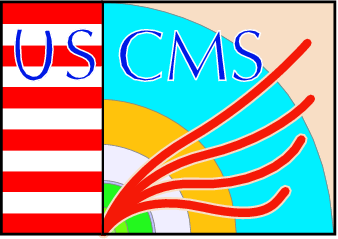
\includegraphics[height=0.6cm]{../../../Graphics/USCMS_logo.png}\hspace{.1cm}
\includegraphics[height=0.75cm]{../../../Graphics/UW_logo.png}}

\begin{document}

% * What is your current amount of resource deployment in HS06, number of
% batch slots and TB of disk available for hosting?
% * What is your roadmap for meeting this FY's deployment goals, which
% are 7.76 kHS06 and 570 TB for hosting?
% * What are your longer-term plans for evolution of your storage element?
% There are currently two approved SE's and one more SE that is undergoing
% development and testing; do you have intentions to change the type of SE
% that you are using?
% * What is your experience with the Tier-2 analysis model of association
% with physics groups?

\begin{frame}
	\titlepage
\end{frame}

\section{Overview}
\begin{frame}
	\tableofcontents
\end{frame}

\section{2009-2010 Facilities Status}
\subsection{Software}
\begin{frame}
\begin{table}
\begin{tabular}{lr}
	\toprule
	Component	 	&	 Software \\
	\midrule
	OS					&	 Scientific Linux 5.3 \\
	Batch			 	&	 Condor 7.4.0 \\
	Storage		 	&	 dCache 1.9.5-8 \\
	Grid				&	 VDT 2.0.0p10 \\
	\bottomrule
\end{tabular}
\caption{2010 Software Status}
\label{2010_software_status}
\end{table}

\begin{itemize}
	\item Software stack increasingly stable from batch to storage
	\item Emphasis on deployment, monitoring
	\item Relocatable OSG installs would (still) be nice
\end{itemize}

\end{frame}

\subsection{Batch}
\begin{frame}
% Use the following to generate N slots:
% condor_status -pool glow.cs.wisc.edu \
%   -constraint 'regexp("g[4-7]n\d+\.hep\.wisc\.edu", Machine)' \
%   -format '%s\n' Machine | wc -l
\begin{table}
\begin{tabular}{lrr}
	\toprule
	CPU Class							&	 HS06		&	Slots \\
	\midrule
	2 x 2.80 GHz Xeon			&	 840		&	 86 \\	% g4-g7, 42 x 20
	2 x 3.00 GHz Xeon			&	 125		&	 10 \\	% g8, 5 x 25
	4 x 1.80 GHz Opteron	&	 1710	 	&	 240 \\	% g9-g10, 57 x 30
	8 x 2.66 GHz Xeon			&	 1976	 	&	 120 \\	% g12, 32 * 61.78
	8 x 3.00 GHz Xeon			&	 2229		&	 260 \\	% g14, 32 * 69.67
	\midrule
	Dedicated							&	 6880		&	 716 \\
	Opportunistic					&	 -			&	 2952 \\
	\bottomrule
\end{tabular}
\caption{2010 Batch Status}
\label{2010_batch_status}
\end{table}

Since last workshop:
\begin{itemize}
	\item Added more opportunistic resources (g16, \ca{}4000 HS06)
	\item Worked to minimize efficiency cost of preemption policies on opportunistic resources
	\item More work on Condor scaling, glide-ins (Dan Bradley)
\end{itemize}
\end{frame}

\begin{frame}
\begin{figure}
	% http://noc.hep.wisc.edu/nrg/condor/pools/GLOW-condor-claimed.1yr.gif
	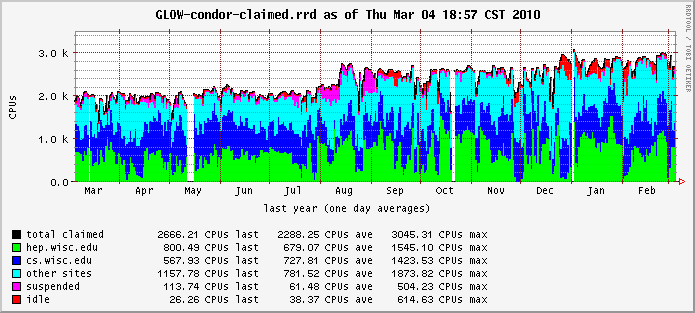
\includegraphics[width=\textwidth]{Graphics/GLOW-condor-claimed-1yr.png}
	\caption{Dedicated and opportunistic slots, 2009-2010}
\end{figure}
\end{frame}

\subsection{Storage}
\begin{frame}
\begin{table}
\begin{tabular}{lr}
	\toprule
	Dedicated			&	 280 TB \\	 % s5, s15 (10 * 24 TB)
	Dual-purpose	&	 200 TB \\	 % rest
	\midrule
	Raw						&	 480 TB \\
	Writable			&	 240 TB \\
	\bottomrule
\end{tabular}
\caption{2010 Storage Status}
\label{2010_storage_status}
\end{table}

Since last workshop:
\begin{itemize}
	\item Purchased 480 TB of dedicated storage; burning in now (online next week)
	\item Upgraded PNFS server hardware, faster RAID (200\% performance improvement)
	\item Developed near real-time dCache replicator ({\tt billingrep})
	\begin{itemize}
		\item No file loss since Summer 2009
	\end{itemize}
\end{itemize}
\end{frame}

\begin{frame}
\begin{figure}
		% http://myosg.grid.iu.edu/wizardse/index?datasource=se&summary_attrs_showservice=on&summary_attrs_showrsvstatus=on&summary_attrs_showfqdn=on&gip_status_attrs_showtestresults=on&gip_status_attrs_showfqdn=on&account_type=daily_hours_byusername&ce_account_type=gip_vo&se_account_type=se_space_free&start_type=specific&start_date=04%2F08%2F2009&end_type=now&end_date=04%2F15%2F2009&facility_10017=on&site_10026=on&r=on&r_24=on&r_27=on&gridtype=on&gridtype_1=on&voown_3=on&active_value=1&disable_value=1
    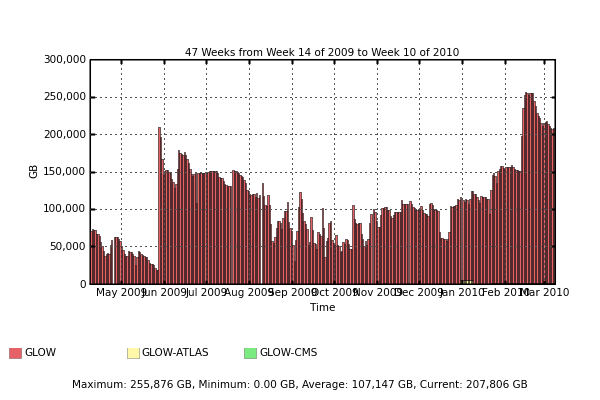
\includegraphics[width=\textwidth]{Graphics/se_space_free.png}
    \caption{dCache usage, 2009-2010}
\end{figure}
\end{frame}

\subsection{Storage tools}
\begin{frame}
\begin{itemize}
	\item Developed many tools to manage dCache
	\begin{itemize}
		\item All code available at \url{http://code.hep.wisc.edu/dcache-tools/}
		\item Includes {\tt dcache_billingrep} (replication service), monitoring scripts
	\end{itemize}
	\item Developed generic Python package to support command line tools
	\begin{itemize}
		\item Documentation and code at \url{http://packages.python.org/pyCLI/}
		\item Used in {\tt dcache-tools}; intended for reuse elsewhere
		\item Provides argument/config parsing, logging, daemonizing, unit/functional test support, etc
		\item ({\tt dcache-tools} uses it)
	\end{itemize}
\end{itemize}
\end{frame}

\subsection{Network and Facilities}
\begin{frame}
\begin{figure}
	% http://stats.net.wisc.edu/cgi-bin/genstatspage.pl?db=r-csscplat-b380-3-core_vl369_bytes&time=1y
	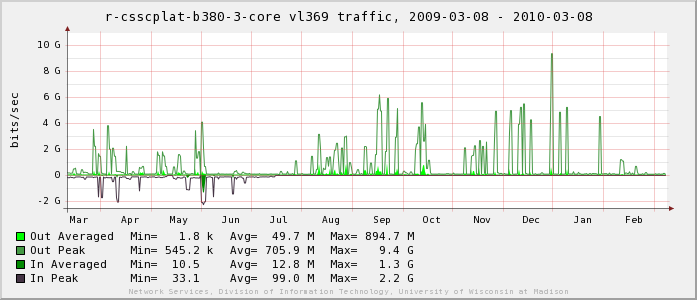
\includegraphics[width=\textwidth]{Graphics/network-1yr.png}
	\caption{Campus WAN usage, 2009-2010}
\end{figure}

\begin{itemize}
	\item Set new campus records
	\item Worked with campus to plan better peering to Nebraska/i2
	\item Added more power to old machine room
	\item Planning for improved cooling in new machine room
\end{itemize}
\end{frame}

\section{2010 Deployment Plans}
\subsection{Batch, storage and software}
\begin{frame}
\begin{table}
\begin{tabular}{lrrr}
	\toprule
	Month					 	&	Storage (raw/writable TB)	&	Slots		& HS06 \\
	\midrule
	March					 	&	480/240										& - 			& - \\
	June						&	256/128										& 256			& 2400 \\
	July						&	Chimera?									&	-				&	- \\
	\midrule
	Current					& 480/240										& 716			& 6880 \\
	New in 2010			&	720/360										& 256 		& 2400 \\
	Total in 2010		&	1200/600									& 972 		& 9280 \\
	\bottomrule
\end{tabular}
\caption{2010 Hardware Deployment Plan}
\label{2010_hardware deployment_plan}
\end{table}

\begin{itemize}
	\item Already close to 2010 milestones
	\item Delay summer purchases to take advantage of 3 TB disks?
	\item Dedicated storage: 8 x E5430 2.66 GHz Xeon, 8 GB RAM, 24 x 2 TB disk, LSI RAID
	\item Dual-purpose: 8 x E5520 2.26 GHz Xeon (\ca{}75 HS06), 24 GB RAM, 4 x 2-3 TB disk
\end{itemize}

\end{frame}

\section{Storage Plans}
\subsection{dCache is dead, long live dCache?}
\begin{frame}
\begin{itemize}
	\item 2009: Participated in early look at Hadoop
	\begin{itemize}
		\item Hardware failures and dCache bugs forced us to switch focus back
	\end{itemize}
	\item Since Summer 2009, storage has been reliable
	\begin{itemize}
		\item Few failures (mostly hardware), but they're well understood
		\item dCache can handle the load at our site
		\item {\tt billingrep} and other local tools worked around many problems
	\end{itemize}
	\item \ldots{}but Hadoop still offers a few things that we really like:
	\begin{itemize}
		\item Chunking
		\item Native replication
		\item Rack awareness
	\end{itemize}
	\item Now that dCache is mostly stable, we have an opportunity to take another look 
	\begin{itemize}
		\item Plan to resurrect small Hadoop test stand Summer 2010
		\item Still need to move to Chimera
		\item Long term? Whatever works
	\end{itemize}
\end{itemize}
\end{frame}

\section{Analysis at Wisconsin}
\begin{frame}
\begin{itemize}
	\item Affiliated with: FWD, TSG (EWK)
	\item Positive feedback from groups, regular use of site for analysis
	\item October Exercise (2009)
	\begin{itemize}
		\item EWK Electron group produced skims at Wisconsin and published data to other T2s
		\item Hosted other Electron data for analysis at Wisconsin; no problems
	\end{itemize}
	\item Quickly find batch problems when supporting global MC production (Ajit Mohapatra)
	\item {\tt farmout} scripts support local analysis (Dan Bradley) 
\end{itemize}
\end{frame}

\end{document}
